\documentclass[11pt,a4paper]{article}
\usepackage{graphicx}
\usepackage{amsmath}
\usepackage{amssymb}
\usepackage{multicol}
\usepackage{tcolorbox}
\usepackage{xcolor}
\usepackage{geometry}
\usepackage{tikz}
\usepackage{array}
\geometry{margin=0.8in}

% Define colors
\definecolor{mlblue}{RGB}{31, 119, 180}
\definecolor{mlorange}{RGB}{255, 127, 14}
\definecolor{mlgreen}{RGB}{44, 160, 44}
\definecolor{mlred}{RGB}{214, 39, 40}
\definecolor{mlpurple}{RGB}{148, 103, 189}

\title{\Large\textbf{Discovery Learning 1: Pattern Hunters}\\
\vspace{0.3em}
\normalsize Finding Natural Groups in Your World}
\author{Machine Learning for Smarter Innovation - Pre-Lecture Activity}
\date{}

\begin{document}
\maketitle
\vspace{-1em}

\begin{tcolorbox}[colback=mlblue!10, colframe=mlblue!50, title=Learning Objectives]
\small
By completing this activity, you will discover:
\begin{itemize}
\item How we naturally group things in everyday life
\item Why different people create different groupings
\item What makes clustering both intuitive and challenging
\end{itemize}
\end{tcolorbox}

\section*{Exercise 1: Festival Band Clustering}
You're organizing a 3-day music festival with 30 bands. You need to group them into time slots and stages. 
Here's your band data:

\begin{center}
\small
\renewcommand{\arraystretch}{0.9}
\begin{tabular}{|l|l|c|c|c|}
\hline
\textbf{Band Name} & \textbf{Genre} & \textbf{Energy (1-10)} & \textbf{Popularity (1-10)} & \textbf{Year Formed} \\
\hline
Electric Storm & Rock & 9 & 7 & 2018 \\
Acoustic Dreams & Folk & 3 & 8 & 2015 \\
Jazz Fusion Five & Jazz & 6 & 5 & 2010 \\
Neon Nights & Electronic & 10 & 9 & 2020 \\
Mountain Echo & Folk & 2 & 6 & 2012 \\
The Algorithms & Electronic & 8 & 8 & 2019 \\
Brass Brigade & Jazz & 5 & 4 & 2008 \\
Digital Pulse & Electronic & 9 & 10 & 2021 \\
Indie Sunrise & Indie & 4 & 7 & 2016 \\
Metal Mayhem & Metal & 10 & 6 & 2017 \\
Smooth Operators & Jazz & 4 & 6 & 2011 \\
Pop Paradise & Pop & 7 & 10 & 2020 \\
Folk Fusion & Folk & 5 & 5 & 2014 \\
Rock Revival & Rock & 8 & 8 & 2013 \\
Synth Symphony & Electronic & 7 & 7 & 2018 \\
Classical Remix & Classical & 3 & 4 & 2009 \\
Punk Patrol & Punk & 10 & 5 & 2019 \\
Blues Brothers 2.0 & Blues & 5 & 6 & 2015 \\
Hip Hop Heroes & Hip-Hop & 8 & 9 & 2021 \\
Country Roads & Country & 4 & 7 & 2016 \\
Latin Groove & Latin & 7 & 8 & 2017 \\
Reggae Rhythm & Reggae & 6 & 6 & 2014 \\
Soul Seekers & Soul & 5 & 7 & 2013 \\
Ambient Atmosphere & Ambient & 1 & 3 & 2011 \\
Disco Dynasty & Disco & 8 & 5 & 2012 \\
Alternative Minds & Alternative & 6 & 8 & 2020 \\
World Wanderers & World & 5 & 4 & 2010 \\
Funk Factory & Funk & 9 & 6 & 2018 \\
R\&B Revolution & R\&B & 6 & 9 & 2019 \\
Experimental Edge & Experimental & 7 & 3 & 2022 \\
\hline
\end{tabular}
\end{center}

\subsection*{Task A: Create Your Groups}
Using the scatter plot below, create 3-5 groups of bands. Draw boundaries around your groups.

\begin{center}
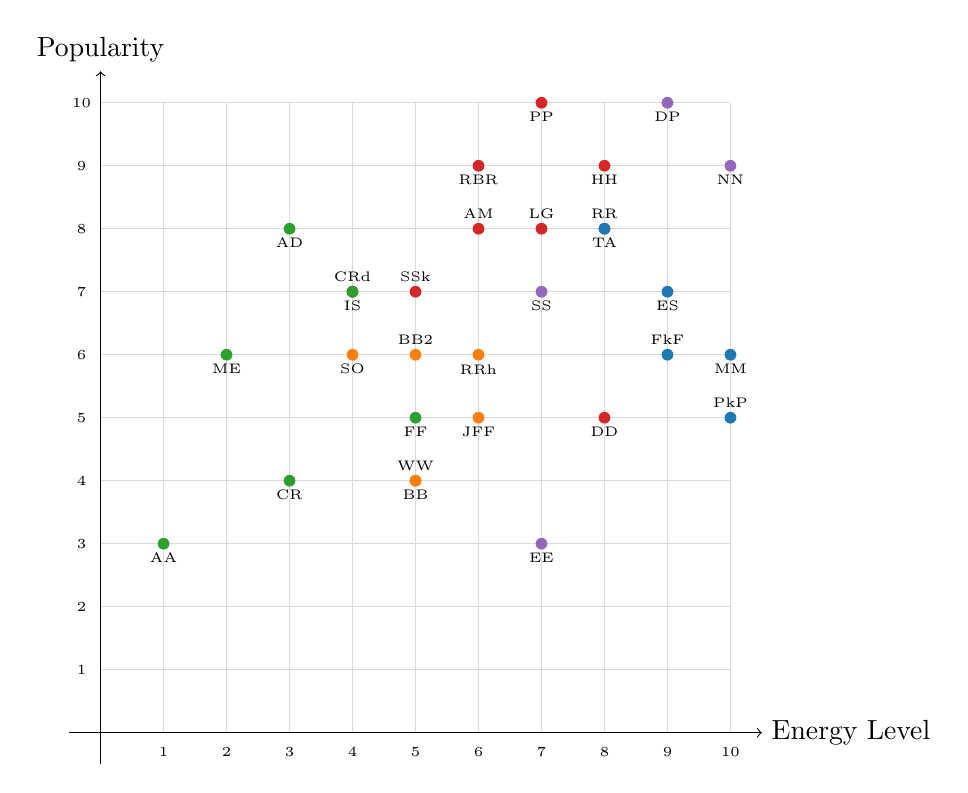
\begin{tikzpicture}[scale=0.8]
% Grid
\draw[gray!30, thin] (0,0) grid (10,10);
% Axes
\draw[->] (-0.5,0) -- (10.5,0) node[right] {Energy Level};
\draw[->] (0,-0.5) -- (0,10.5) node[above] {Popularity};
% Numbers
\foreach \x in {1,2,3,4,5,6,7,8,9,10}
    \node at (\x,-0.3) {\tiny\x};
\foreach \y in {1,2,3,4,5,6,7,8,9,10}
    \node at (-0.3,\y) {\tiny\y};

% Plot points (abbreviated names)
\node[circle, fill=mlblue, inner sep=1.5pt] at (9,7) {};
\node[below, font=\tiny] at (9,7) {ES};
\node[circle, fill=mlgreen, inner sep=1.5pt] at (3,8) {};
\node[below, font=\tiny] at (3,8) {AD};
\node[circle, fill=mlorange, inner sep=1.5pt] at (6,5) {};
\node[below, font=\tiny] at (6,5) {JFF};
\node[circle, fill=mlpurple, inner sep=1.5pt] at (10,9) {};
\node[below, font=\tiny] at (10,9) {NN};
\node[circle, fill=mlgreen, inner sep=1.5pt] at (2,6) {};
\node[below, font=\tiny] at (2,6) {ME};
\node[circle, fill=mlpurple, inner sep=1.5pt] at (8,8) {};
\node[below, font=\tiny] at (8,8) {TA};
\node[circle, fill=mlorange, inner sep=1.5pt] at (5,4) {};
\node[below, font=\tiny] at (5,4) {BB};
\node[circle, fill=mlpurple, inner sep=1.5pt] at (9,10) {};
\node[below, font=\tiny] at (9,10) {DP};
\node[circle, fill=mlred, inner sep=1.5pt] at (4,7) {};
\node[below, font=\tiny] at (4,7) {IS};
\node[circle, fill=mlblue, inner sep=1.5pt] at (10,6) {};
\node[below, font=\tiny] at (10,6) {MM};
\node[circle, fill=mlorange, inner sep=1.5pt] at (4,6) {};
\node[below, font=\tiny] at (4,6) {SO};
\node[circle, fill=mlred, inner sep=1.5pt] at (7,10) {};
\node[below, font=\tiny] at (7,10) {PP};
\node[circle, fill=mlgreen, inner sep=1.5pt] at (5,5) {};
\node[below, font=\tiny] at (5,5) {FF};
\node[circle, fill=mlblue, inner sep=1.5pt] at (8,8) {};
\node[above, font=\tiny] at (8,8) {RR};
\node[circle, fill=mlpurple, inner sep=1.5pt] at (7,7) {};
\node[below, font=\tiny] at (7,7) {SS};
\node[circle, fill=mlgreen, inner sep=1.5pt] at (3,4) {};
\node[below, font=\tiny] at (3,4) {CR};
\node[circle, fill=mlblue, inner sep=1.5pt] at (10,5) {};
\node[above, font=\tiny] at (10,5) {PkP};
\node[circle, fill=mlorange, inner sep=1.5pt] at (5,6) {};
\node[above, font=\tiny] at (5,6) {BB2};
\node[circle, fill=mlred, inner sep=1.5pt] at (8,9) {};
\node[below, font=\tiny] at (8,9) {HH};
\node[circle, fill=mlgreen, inner sep=1.5pt] at (4,7) {};
\node[above, font=\tiny] at (4,7) {CRd};
\node[circle, fill=mlred, inner sep=1.5pt] at (7,8) {};
\node[above, font=\tiny] at (7,8) {LG};
\node[circle, fill=mlorange, inner sep=1.5pt] at (6,6) {};
\node[below, font=\tiny] at (6,6) {RRh};
\node[circle, fill=mlred, inner sep=1.5pt] at (5,7) {};
\node[above, font=\tiny] at (5,7) {SSk};
\node[circle, fill=mlgreen, inner sep=1.5pt] at (1,3) {};
\node[below, font=\tiny] at (1,3) {AA};
\node[circle, fill=mlred, inner sep=1.5pt] at (8,5) {};
\node[below, font=\tiny] at (8,5) {DD};
\node[circle, fill=mlred, inner sep=1.5pt] at (6,8) {};
\node[above, font=\tiny] at (6,8) {AM};
\node[circle, fill=mlorange, inner sep=1.5pt] at (5,4) {};
\node[above, font=\tiny] at (5,4) {WW};
\node[circle, fill=mlblue, inner sep=1.5pt] at (9,6) {};
\node[above, font=\tiny] at (9,6) {FkF};
\node[circle, fill=mlred, inner sep=1.5pt] at (6,9) {};
\node[below, font=\tiny] at (6,9) {RBR};
\node[circle, fill=mlpurple, inner sep=1.5pt] at (7,3) {};
\node[below, font=\tiny] at (7,3) {EE};
\end{tikzpicture}
\end{center}

\textbf{Your grouping criteria:} \underline{\hspace{8cm}}

\newpage

\section*{Exercise 2: Real-World Pattern Hunt}

\subsection*{Task B: Find Clustering in Your Life}
Identify how clustering happens in these everyday scenarios:

\begin{center}
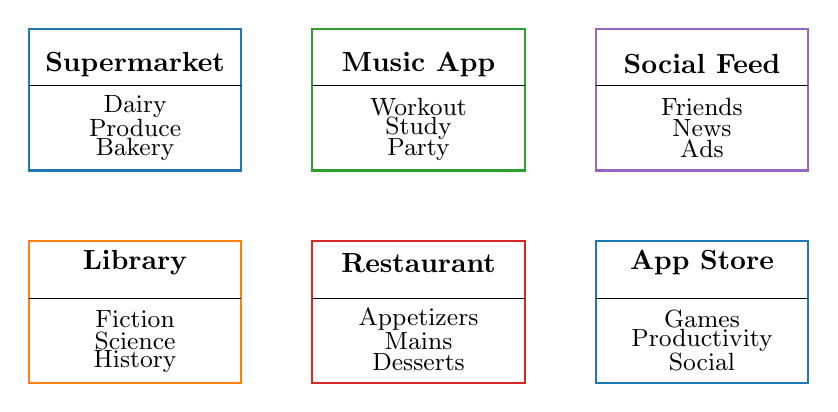
\begin{tikzpicture}[scale=0.9]
% Supermarket
\draw[thick, mlblue] (0,0) rectangle (3,2);
\node at (1.5,1.5) {\textbf{Supermarket}};
\draw (0,1.2) -- (3,1.2);
\node[font=\small] at (1.5,0.9) {Dairy};
\node[font=\small] at (1.5,0.6) {Produce};
\node[font=\small] at (1.5,0.3) {Bakery};

% Spotify
\draw[thick, mlgreen] (4,0) rectangle (7,2);
\node at (5.5,1.5) {\textbf{Music App}};
\draw (4,1.2) -- (7,1.2);
\node[font=\small] at (5.5,0.9) {Workout};
\node[font=\small] at (5.5,0.6) {Study};
\node[font=\small] at (5.5,0.3) {Party};

% Social Media
\draw[thick, mlpurple] (8,0) rectangle (11,2);
\node at (9.5,1.5) {\textbf{Social Feed}};
\draw (8,1.2) -- (11,1.2);
\node[font=\small] at (9.5,0.9) {Friends};
\node[font=\small] at (9.5,0.6) {News};
\node[font=\small] at (9.5,0.3) {Ads};

% Library
\draw[thick, mlorange] (0,-3) rectangle (3,-1);
\node at (1.5,-1.3) {\textbf{Library}};
\draw (0,-1.8) -- (3,-1.8);
\node[font=\small] at (1.5,-2.1) {Fiction};
\node[font=\small] at (1.5,-2.4) {Science};
\node[font=\small] at (1.5,-2.7) {History};

% Restaurant Menu
\draw[thick, mlred] (4,-3) rectangle (7,-1);
\node at (5.5,-1.3) {\textbf{Restaurant}};
\draw (4,-1.8) -- (7,-1.8);
\node[font=\small] at (5.5,-2.1) {Appetizers};
\node[font=\small] at (5.5,-2.4) {Mains};
\node[font=\small] at (5.5,-2.7) {Desserts};

% App Store
\draw[thick, mlblue] (8,-3) rectangle (11,-1);
\node at (9.5,-1.3) {\textbf{App Store}};
\draw (8,-1.8) -- (11,-1.8);
\node[font=\small] at (9.5,-2.1) {Games};
\node[font=\small] at (9.5,-2.4) {Productivity};
\node[font=\small] at (9.5,-2.7) {Social};
\end{tikzpicture}
\end{center}

\textbf{Pick one example above. What features determine the groups?}
\begin{itemize}
\item Example chosen: \underline{\hspace{3cm}}
\item Feature 1: \underline{\hspace{5cm}}
\item Feature 2: \underline{\hspace{5cm}}
\item Feature 3: \underline{\hspace{5cm}}
\end{itemize}

\begin{tcolorbox}[colback=mlorange!10, colframe=mlorange!50, title=Discovery Moment]
\textbf{What happens when something doesn't fit clearly into any group?}\\
\vspace{0.5em}
Example: Is a tomato in fruits or vegetables? Is a podcast app entertainment or education?\\
\vspace{0.5em}
Your example: \underline{\hspace{8cm}}\\
\vspace{0.3em}
How did you decide: \underline{\hspace{7cm}}
\end{tcolorbox}

\section*{Reflection Questions}
\begin{enumerate}
\item \textbf{Compare with a partner:} Did you create the same band groups? Why or why not?\\
\vspace{0.3em}
\underline{\hspace{13cm}}\\
\underline{\hspace{13cm}}

\item \textbf{Scale challenge:} You grouped 30 bands. Imagine having 5,000 bands to organize. What would make this difficult?\\
\vspace{0.3em}
\underline{\hspace{13cm}}\\
\underline{\hspace{13cm}}

\item \textbf{Feature importance:} If you could only use ONE feature (energy OR popularity), which would create better groups? Why?\\
\vspace{0.3em}
\underline{\hspace{13cm}}\\
\underline{\hspace{13cm}}
\end{enumerate}

\begin{tcolorbox}[colback=mlpurple!10, colframe=mlpurple!50, title=Prepare for Next Class]
In our next lecture, you'll learn how computers can automatically find these patterns in massive datasets with thousands of items and dozens of features. Think about: What rules could you give a computer to group things the way you did?
\end{tcolorbox}

\end{document}